\documentclass[a4paper]{article}

%use the english line for english reports
%usepackage[english]{babel}
\usepackage[portuguese]{babel}
\usepackage[utf8]{inputenc}
\usepackage{indentfirst}
\usepackage{graphicx}
\usepackage{verbatim}


\begin{document}

\setlength{\textwidth}{16cm}
\setlength{\textheight}{22cm}

\title{\Huge\textbf{Jogo de Tabuleiro - Campo Bello}\linebreak\linebreak\linebreak
\Large\textbf{Relatório Intercalar}\linebreak\linebreak
\linebreak\linebreak

\includegraphics[scale=0.1]{feup-logo.png}\linebreak\linebreak
\linebreak\linebreak
\Large{Mestrado Integrado em Engenharia Informática e Computação} \linebreak\linebreak
\Large{Programação em Lógica}\linebreak
}

\author{\textbf{Grupo 04:}\\
João Nuno Fonseca Seixas - 201505648 \\
Renato Alexandre Sousa Campos - 201504942\\
\linebreak\linebreak \\
 \\ Faculdade de Engenharia da Universidade do Porto \\ Rua Roberto Frias, s\/n, 4200-465 Porto, Portugal \linebreak\linebreak\linebreak
\linebreak\linebreak\vspace{1cm}}

\maketitle
\thispagestyle{empty}

%************************************************************************************************
%************************************************************************************************

\newpage

%Todas as figuras devem ser referidas no texto. %\ref{fig:codigoFigura}
%
%%Exemplo de código para inserção de figuras
%%\begin{figure}[h!]
%%\begin{center}
%%escolher entre uma das seguintes três linhas:
%%\includegraphics[height=20cm,width=15cm]{path relativo da imagem}
%%\includegraphics[scale=0.5]{path relativo da imagem}
%%\includegraphics{path relativo da imagem}
%%\caption{legenda da figura}
%%\label{fig:codigoFigura}
%%\end{center}
%%\end{figure}
%
%
%\textit{Para escrever em itálico}
%\textbf{Para escrever em negrito}
%Para escrever em letra normal
%``Para escrever texto entre aspas''
%
%Para fazer parágrafo, deixar uma linha em branco.
%
%Como fazer bullet points:
%\begin{itemize}
	%\item Item1
	%\item Item2
%\end{itemize}
%
%Como enumerar itens:
%\begin{enumerate}
	%\item Item 1
	%\item Item 2
%\end{enumerate}
%
%\begin{quote}``Isto é uma citação''\end{quote}


%%%%%%%%%%%%%%%%%%%%%%%%%%
\section{O Jogo Campo Bello}

Campo Bello é um jogo que pode ser jogado de 2 a 4 jogadores. Tem inspiração no jogo clássico "Resta Um" ou "Peg Solitaire" em Inglês. É um jogo ainda recente, criado em 2017.
Para ganhar, um jogador deve tentar remover todas as suas peças do tabuleiro antes dos adversários.
O tabuleiro consiste em 4 triângulos que rodeiam um diamante central. Os triângulos correspodem às áreas iniciais de cada jogador. As peças são removidas ao saltar:  saltar uma peça nossa causa a remoção da peça que foi saltada; saltar uma peça adversária permite-nos remover uma peça nossa do tabuleiro.
Na variante de apenas 2 jogadores, que vai ser implementada, os jogadores ficam com triângulos opostos e jogam alternadamente.
É também possível executar saltos duplos e triplos numa só jogada.
No fim do jogo cada jogador pontua 1 ponto por cada uma das suas peças fora da área inicial e 3 pontos por cada uma das suas peças dentro da sua área inicial.
O jogador com menos pontos ganha!\linebreak\linebreak
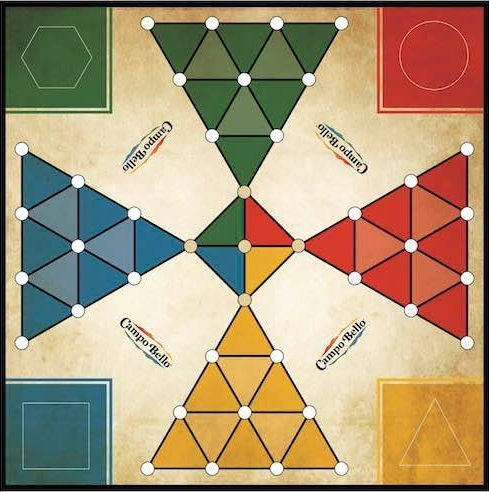
\includegraphics[scale=0.9]{originalBoard.png}\linebreak\linebreak
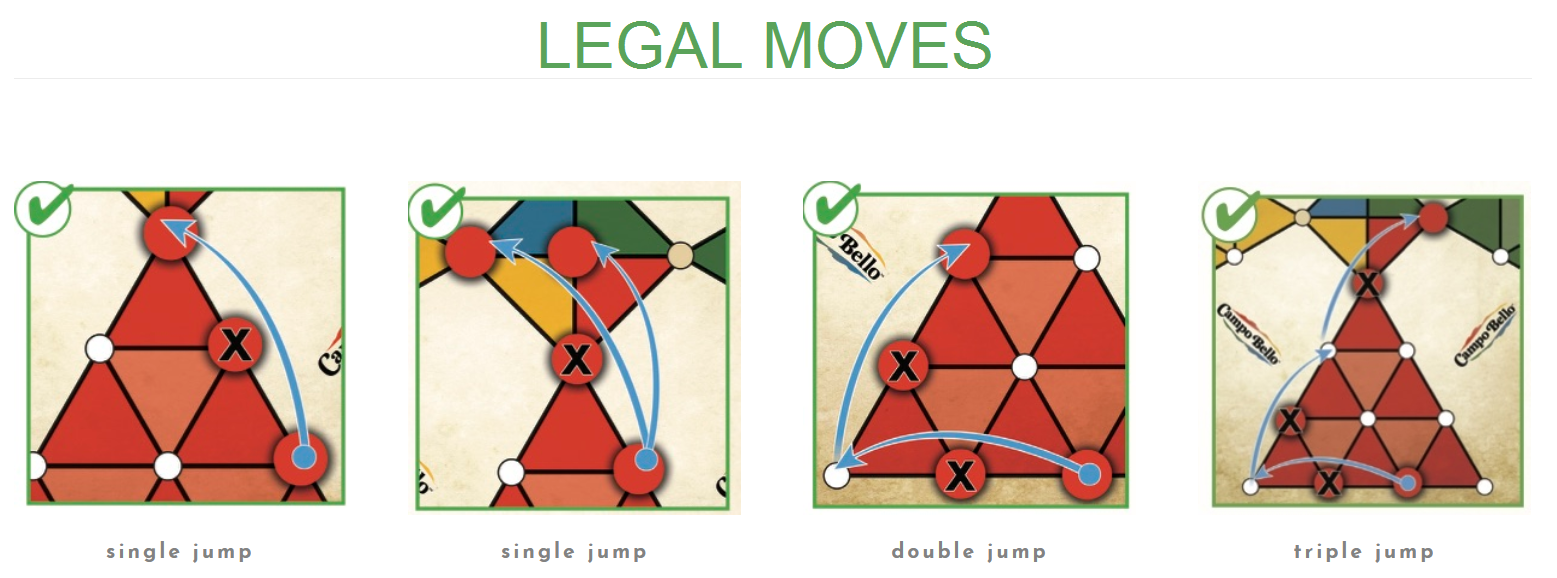
\includegraphics[scale=0.3]{legalMoves.PNG}\linebreak\linebreak
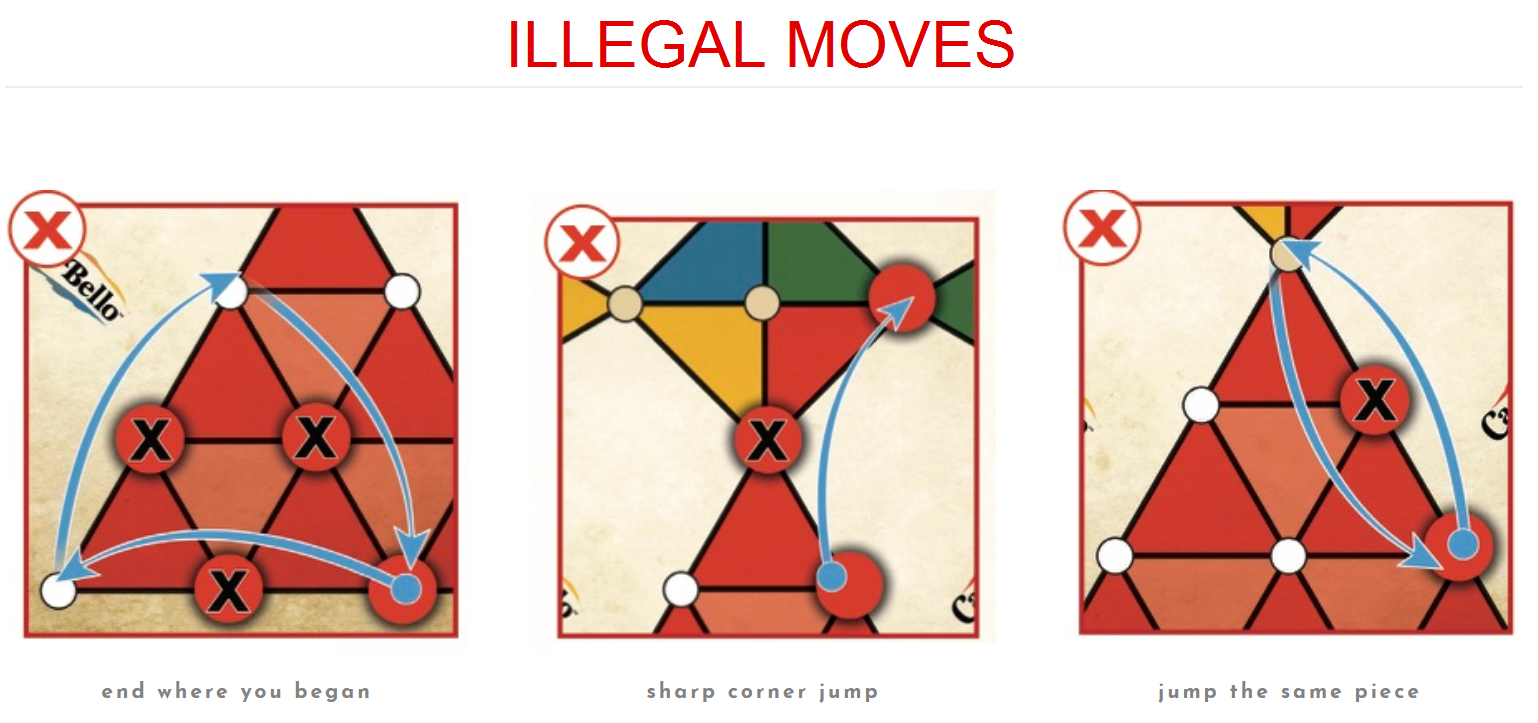
\includegraphics[scale=0.3]{illegalMoves.PNG}\linebreak\linebreak
%Devem ser incluidas imagens apropriadas para explicar o funcionamento do jogo.
%Devem ser incluidas as fontes de informação (e.g. URLs em rodapé).
http://www.campobellogame.com/


%%%%%%%%%%%%%%%%%%%%%%%%%%
\section{Representação do Estado do Jogo}

%Descrever a forma de representação do estado do tabuleiro (tipicamente uma lista de listas), com exemplificação em Prolog de posições iniciais do jogo, posições intermédias e finais, acompanhadas de imagens ilustrativas.

O estado do jogo é representado por 2 listas que identificam em que posições do tabuleiro estão as peças de cada jogador (1 lista para cada jogador). As peças de cada jogador sáo designadas em Inglês por "movers".\linebreak

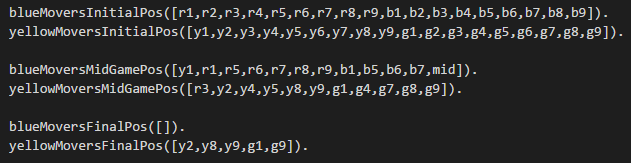
\includegraphics[scale=0.7]{gameStates.PNG}\linebreak\linebreak
Imagens do tabuleiro nos respetivos estados de jogo (inicial, intermédio e final):\linebreak

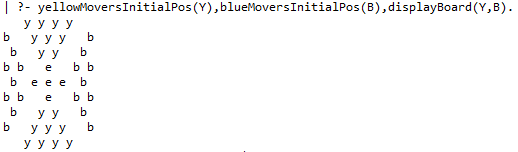
\includegraphics[scale=1]{initialBoard.PNG}\linebreak\linebreak

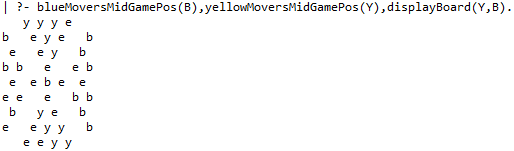
\includegraphics[scale=1]{midGameBoard.PNG}\linebreak\linebreak

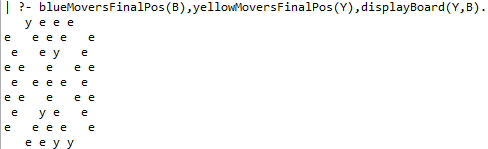
\includegraphics[scale=1]{endGameBoard.PNG}\linebreak\linebreak
Com o decorrer do jogo as listas perdem elementos. O estado final do jogo é alcançado quando uma das listas estiver vazia ou quando não houver mais jogadas possíveis para os 2 jogadores.


%%%%%%%%%%%%%%%%%%%%%%%%%%
\section{Visualização do Tabuleiro}

O predicado para visualização do tabuleiro é muito específico, visto que cada linha tem de ser impressa de maneira diferente.

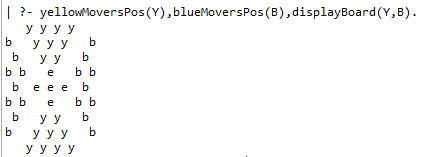
\includegraphics[scale=1]{printBoard.PNG}\linebreak\linebreak
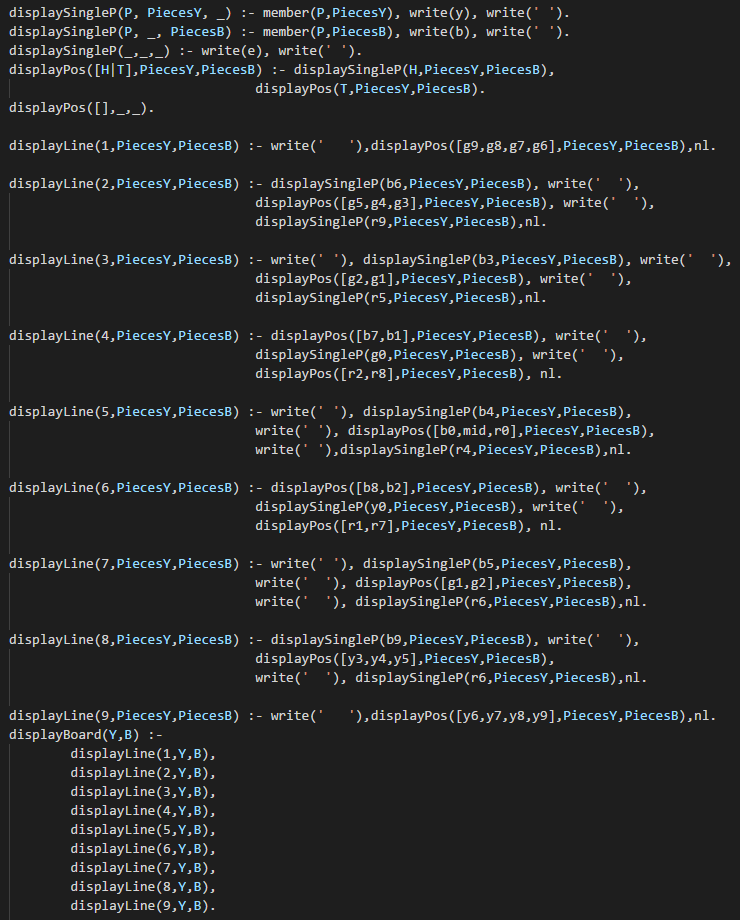
\includegraphics[scale=0.6]{displayBoard.PNG}\linebreak\linebreak




%%%%%%%%%%%%%%%%%%%%%%%%%%
\section{Movimentos}

\begin{flushleft} 
\hspace{5mm} \textbf{Fazer uma jogada:}\linebreak
\textit {makePlay(Player,Yi,Bi,InitialPos,JumpPos,FinalPos,Yo,Bo)}\linebreak

\hspace{5mm} \textbf{Verificar se é válida:}\linebreak
\textit{isValid(Player,Yi,Bi,InitialPos,JumpPos,FinalPos)}\linebreak

\hspace{5mm} \textbf{Mover a peça:}\linebreak
\textit{move(Yi,Bi,InitialPos,JumpPos,FinalPos,Yo,Bo)}\linebreak
\end{flushleft}



\end{document}
